\begin{normalsize}
\textbf{Statistical Terminology.} A random variable $X$ is precisely
defined by its \textit{cumulative distribution function} (CDF) $F_X$
and the derivative of the CDF, the \textit{probability density
  function} (PDF) $f_X.$ For any possible value $x$ of $X$, the
\textit{percentile} of $x$ is $100$ $F_X(x)$, the percentage of values
drawn from $X$ that would be less than or equal to $x$ as the number
of samples tends towards infinity. The \textit{quartiles} of $X$ are
its $25$-th, $50$-th (median), and $75$-th percentiles. The absolute
difference between the median and an adjacent quartile is an
\textit{interquartile range}. Given an independent and identically
distributed sample from $X$ and presuming that $X$ has finite mean and
variance, a \textit{confidence interval} can be drawn about any
percentile estimated from the sample. A \textit{confidence interval}
describes the probability that a value lies within an interval. The
\textit{null hypothesis} is a statement (derived from some test
statistic) that the expected value of the observed statistic is equal
to an assumed population statistic. The $p$ value is the probability
of observing a given statistic if the \textit{null hypothesis} is
true. For a more detailed introduction to statistics and 
related terminology, see the work of Navidi \cite{navidi_2015}.

\vspace{4mm}
\noindent \textbf{Raw Numerical Results.} The tables that follow show the
precise experimental results for all data sets presented in Section
\ref{sec:data}. The tests were all run serially on an otherwise idle
machine with a CentOS 6.10 operating system and an Intel i7-3770 CPU
operating at 3.4 GHz. The detailed performance results in the tables
that follow are very much dependent on the problem and the algorithm
implementation (e.g., some codes are TOMS software, some industry
distributions, and others are from conference paper venues). Different
typeface is used to show best performers, however not much
significance should be attached to ranking algorithms based on small
time (millisecond) differences. The results serve as a demonstration
of conceptual validity.

\end{normalsize}

\begin{figure}[h]
  \centering
  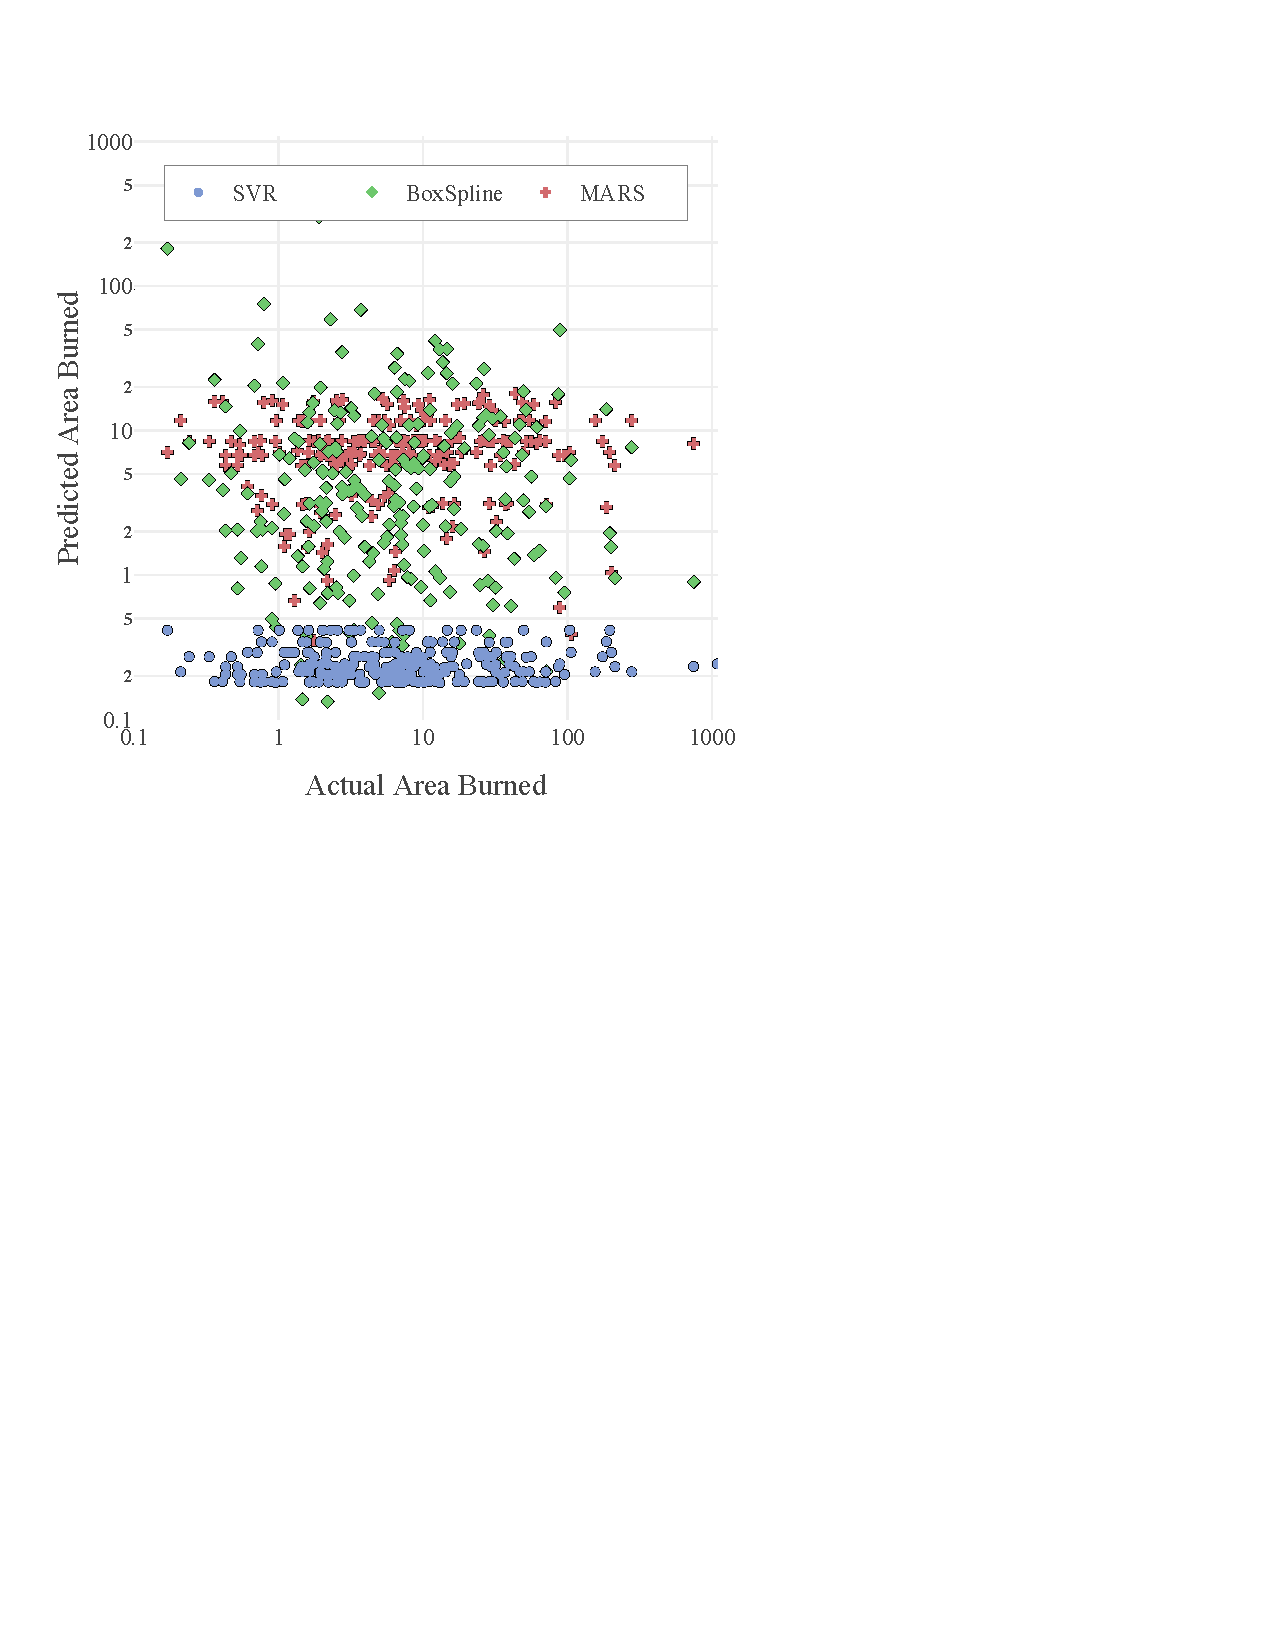
\includegraphics[width=0.45\textwidth,]{Figures/NA/scatter_forestfires.pdf}
  \hspace{.6cm}
  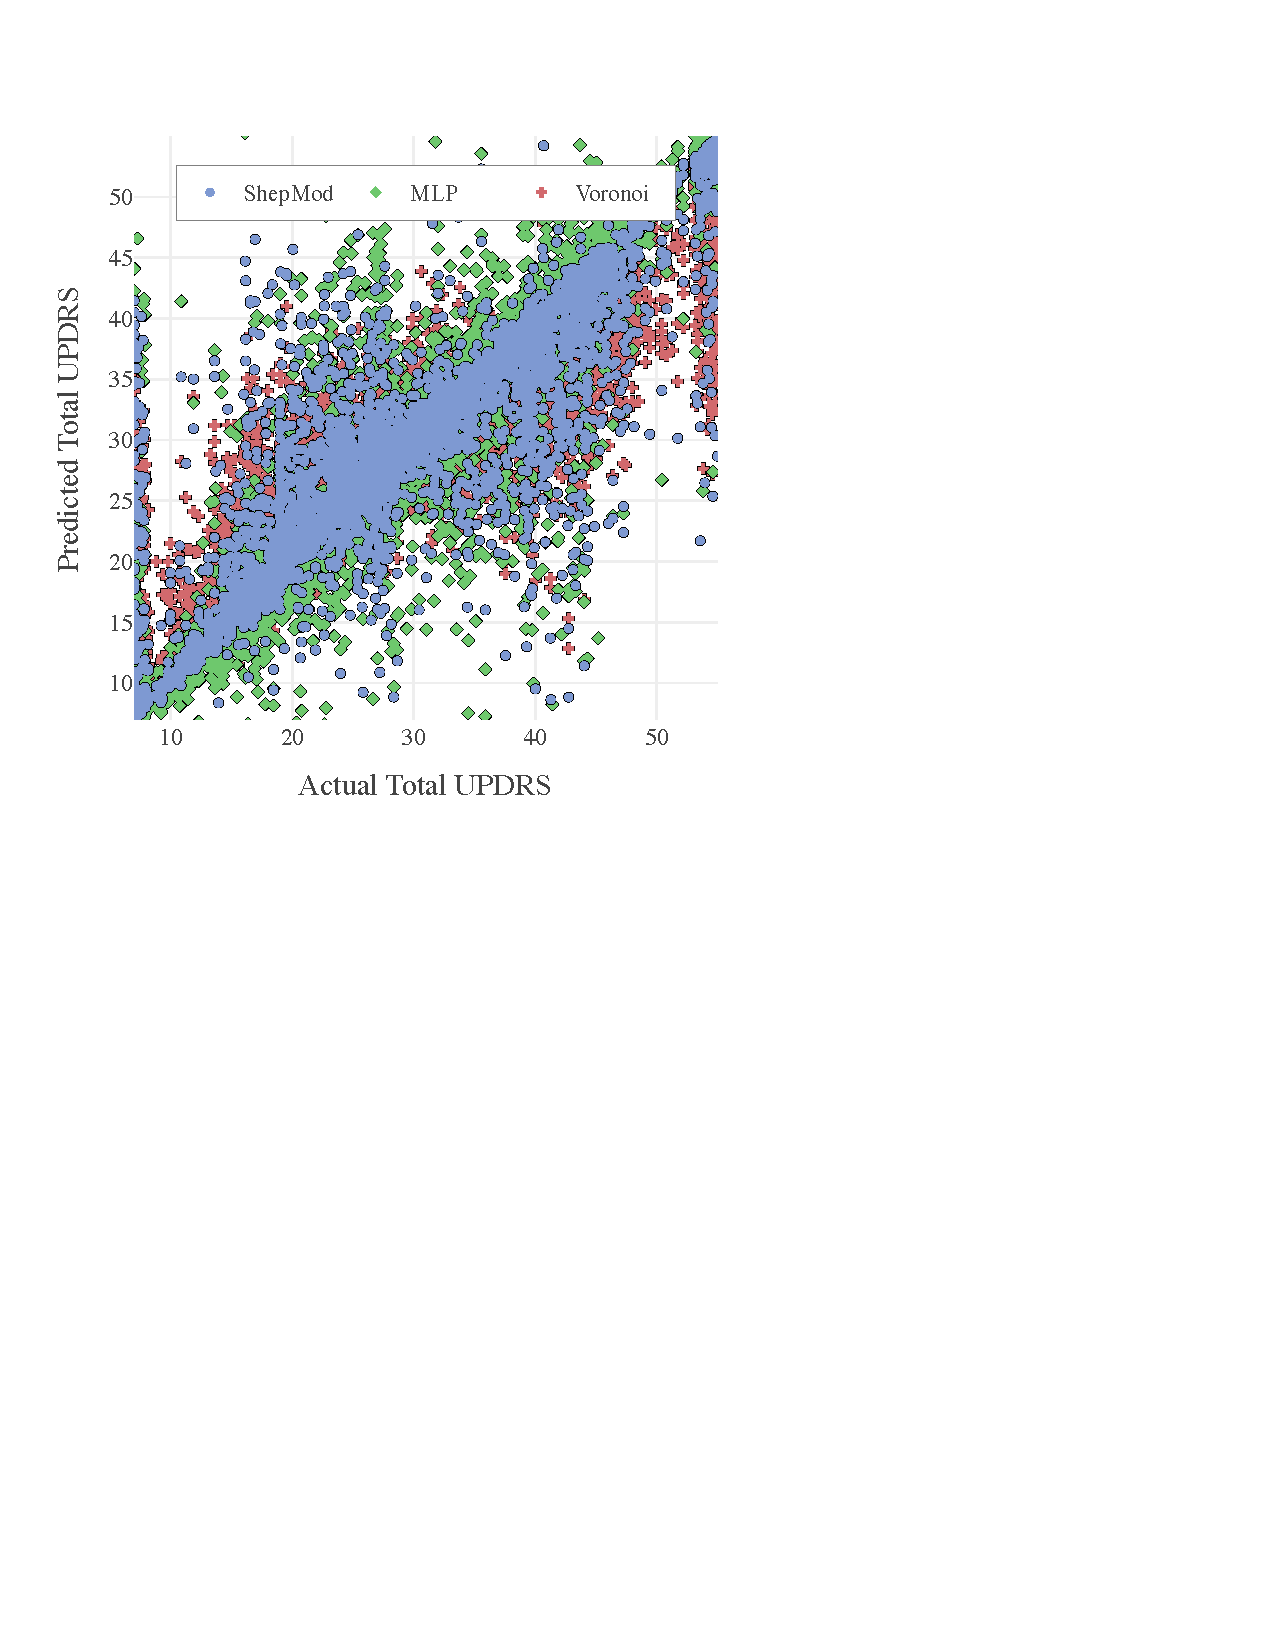
\includegraphics[width=0.45\textwidth,]{Figures/NA/scatter_parkinsons.pdf}
  \vspace{.6cm}

  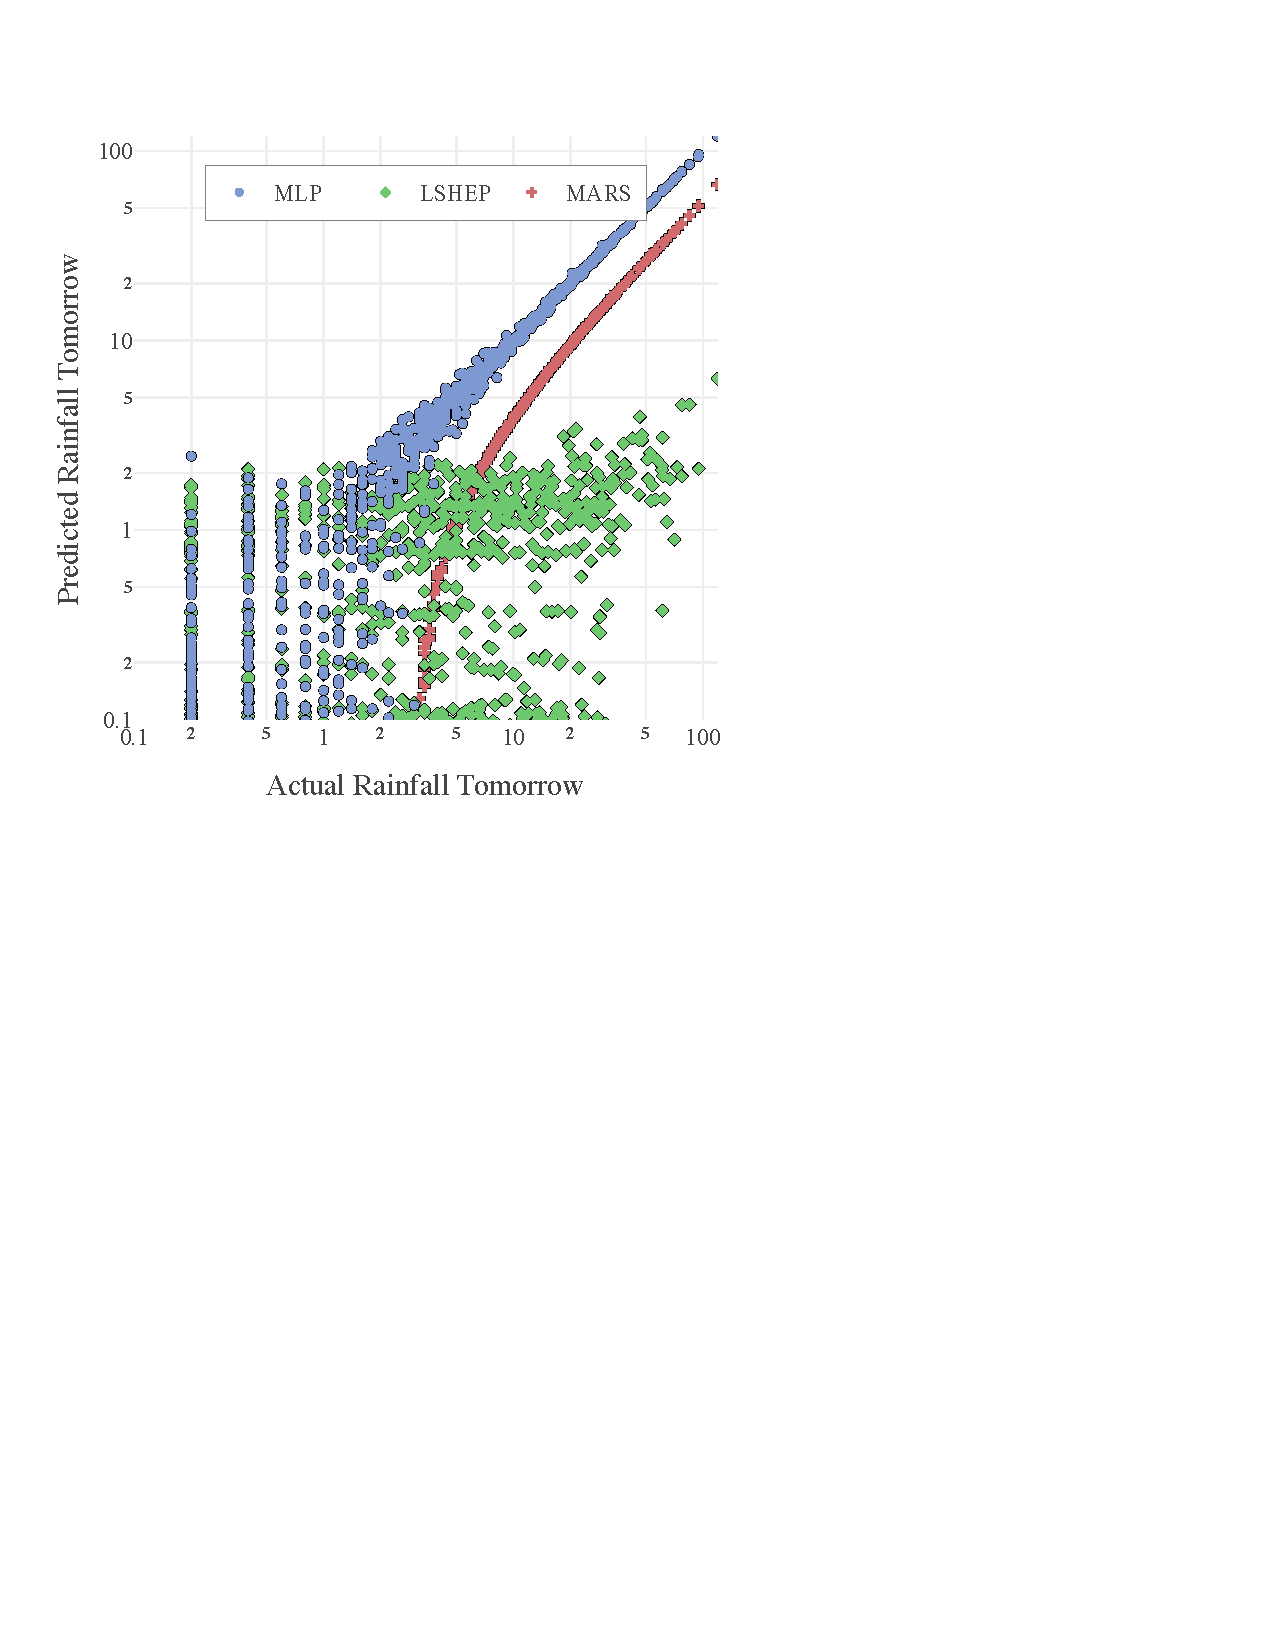
\includegraphics[width=0.45\textwidth,]{Figures/NA/scatter_weather.pdf}
  \hspace{.6cm}
  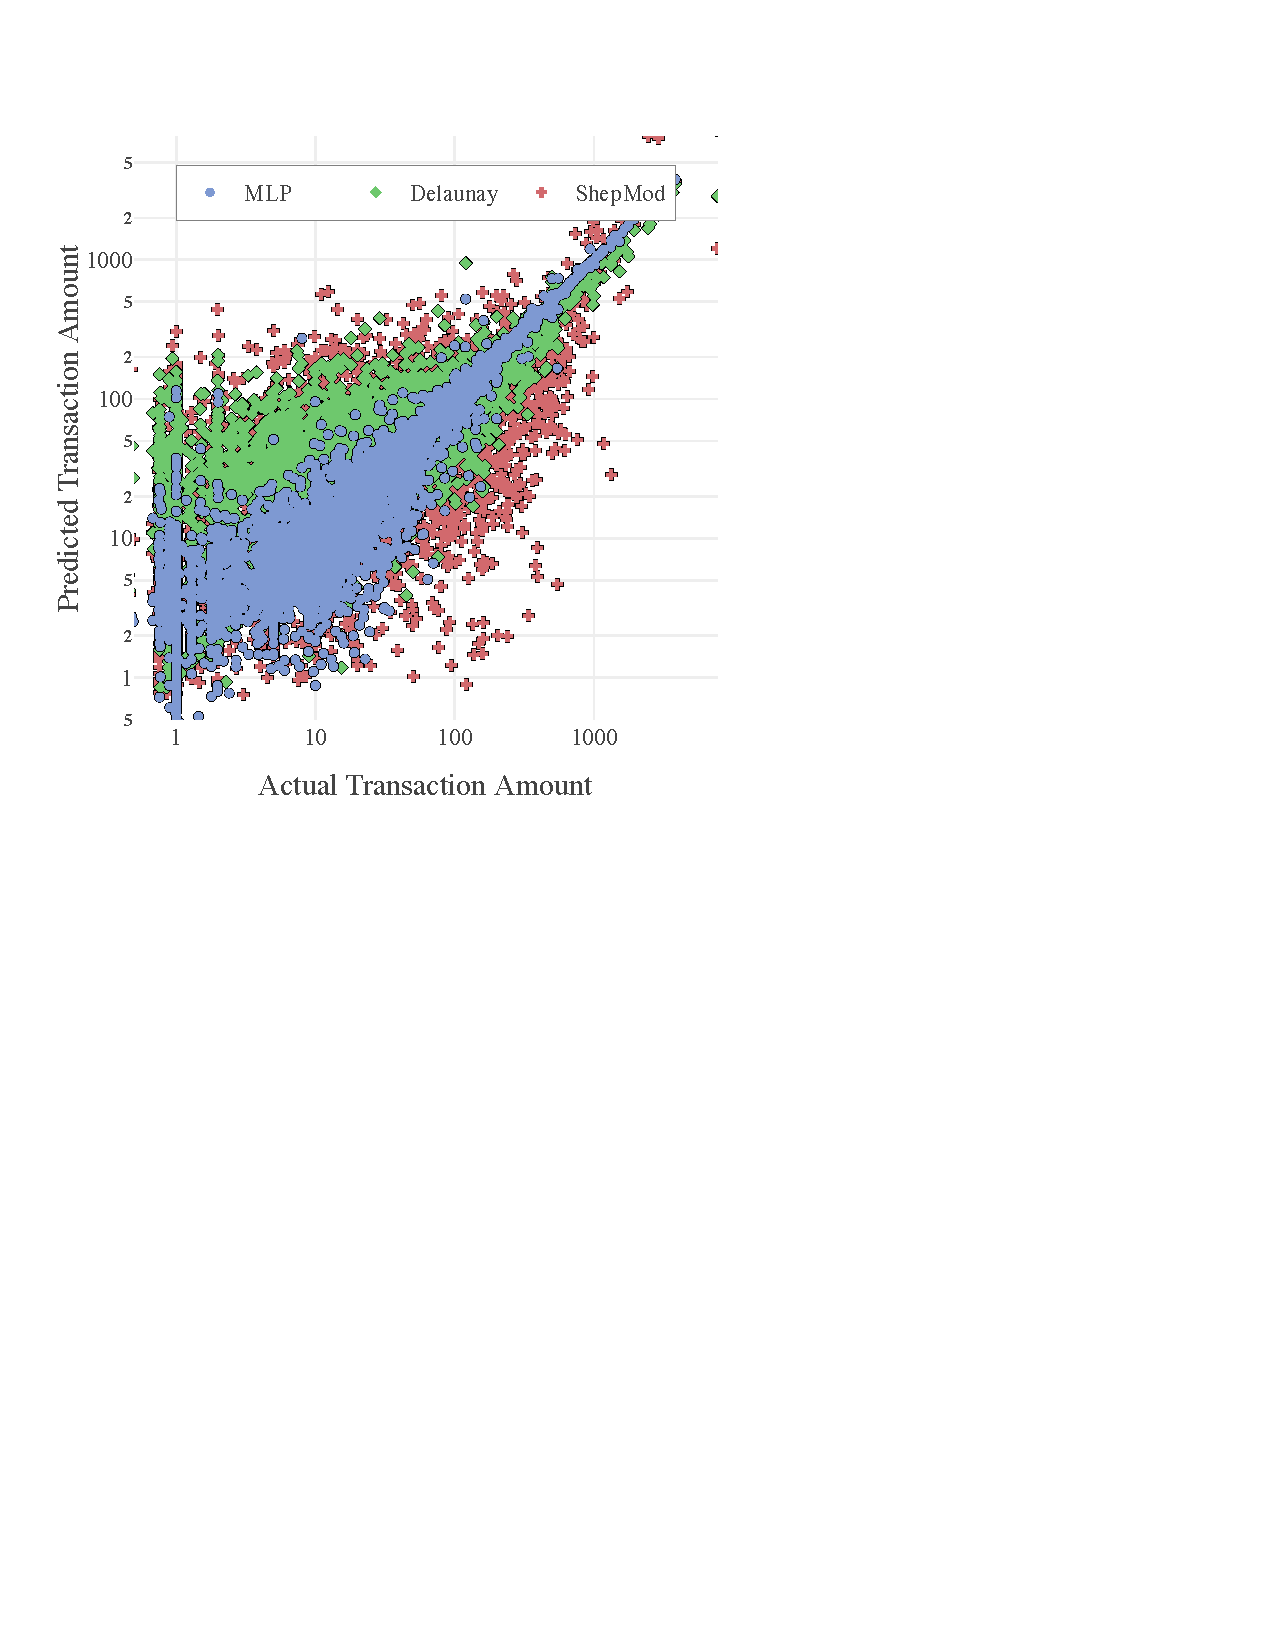
\includegraphics[width=0.45\textwidth,]{Figures/NA/scatter_creditcard.pdf}
  \vspace{.3cm}

  \caption{Scatter plots for predicted versus actual values for the
    top three models on each of the four real valued approximation
    problems. Top left is forest fire data, top right is Parkinson's
    data, bottom left is rainfall data, and bottom right is credit
    card transaction data. The blue circles correspond to the best
    model, green diamonds to the second best, and red crosses to the
    third best model for each data set. There are a large of number of
    0-valued entries in the forest fire and rainfall data sets that
    are not included in the visuals making the true ranking of the
    models appear to disagree with the observed outcomes.}
  \label{fig:scatter_plots}
\end{figure}


\begin{table}[H]
  \centering
  \begin{tabular}{c|r@{.}l|r@{.}l|r@{.}l|r@{.}l|r@{.}l}
    \hline
    Algorithm & \multicolumn{2}{c}{Min}       & \multicolumn{2}{c}{$25^{th}$} & \multicolumn{2}{c}{$50^{th}$} & \multicolumn{2}{c}{$75^{th}$} & \multicolumn{2}{c}{Max}\\
    \hline
    MARS      & $0$&$00984$                   & $3$&$11$                      & $7$&$01$                      & $\mathit{11}$&$\mathit{7}$    & $1090$&$0$\\
    SVR       & $0$&$0118$                    & $\mathbf{0}$&$\mathbf{615}$   & $\mathbf{0}$&$\mathbf{931}$   & $\mathbf{5}$&$\mathbf{89}$    & $1090$&$0$\\
    MLP       & $0$&$0426$                    & $2$&$63$                      & $5$&$27$                      & $14$&$0$                      & $1090$&$0$\\
    Delaunay  & $\mathbf{0}$&$\mathbf{0}$     & $1$&$98$                      & $5$&$37$                      & $13$&$1$                      & $\mathit{1080}$&$\mathit{0}$\\
    ShepMod   & $\mathbf{0}$&$\mathbf{0}$     & $1$&$93$                      & $6$&$27$                      & $16$&$0$                      & $1090$&$0$\\
    LSHEP     & $0$&$04$                      & $2$&$17$                      & $8$&$87$                      & $19$&$1$                      & $\mathbf{1070}$&$\mathbf{0}$\\
    Voronoi   & $\mathit{0}$&$\mathit{00982}$ & $3$&$65$                      & $7$&$56$                      & $15$&$6$                      & $1090$&$0$\\
    BoxSpline & $\mathbf{0}$&$\mathbf{0}$     & $\mathit{1}$&$\mathit{27}$    & $\mathit{4}$&$\mathit{61}$    & $12$&$6$                      & $1090$&$0$\\
    \hline
  \end{tabular}
  \caption{This numerical data accompanies the visual provided in
    Figure \ref{fig:error-forest-fire}. The columns of absolute error
    percentiles correspond to the minimum, first quartile, median,
    third quartile, and maximum absolute errors respectively. The
    minimum of each column is boldface, while the second lowest value
    is italicized. All values are rounded to three significant
    digits.}
  \vspace{.2cm}
  \label{table:error-forest-fire}

  \begin{tabular}{|c|r@{.}l| c |r@{.}l|r@{.}l|r@{.}l|}
    \cline{1-3}\cline{5-10}
    Algorithm & \multicolumn{2}{c|}{\% Best}   &  & \multicolumn{2}{c|}{Fit/Prep. Time (s)} & \multicolumn{2}{c|}{App. Time (s)} & \multicolumn{2}{c|}{Total App. Time (s)}\\
    \cline{1-3}\cline{5-10}
    MARS      & \quad$7$&$3$                   &  & \quad\quad$29$&$1$                      & \quad$0$&$00137$                   & \quad\quad\quad$0$&$0686$\\
    SVR       & $\mathbf{78}$&$\mathbf{0}$     &  & $\mathbf{0}$&$\mathbf{00584}$           & $\mathit{0}$&$\mathit{0000620}$    & $\mathit{0}$&$\mathit{00310}$\\
    MLP       & $0$&$0$                        &  & $32$&$8$                                & $0$&$000871$                       & $0$&$0436$\\
    Delaunay  & $0$&$2$                        &  & $0$&$0151$                              & $0$&$0234$                         & $1$&$18$\\
    ShepMod   & $2$&$0$                        &  & $\mathit{0}$&$\mathit{00634}$           & $0$&$0000644$                      & $0$&$00322$\\
    LSHEP     & $5$&$1$                        &  & $0$&$0275$                              & $\mathbf{0}$&$\mathbf{0000463}$    & $\mathbf{0}$&$\mathbf{00231}$\\
    Voronoi   & $0$&$0$                        &  & $0$&$0152$                              & $0$&$000396$                       & $0$&$0198$\\
    BoxSpline & $\mathit{9}$&$\mathit{7}$      &  & $0$&$00724$                             & $0$&$0000978$                      & $0$&$00489$\\
    \cline{1-3}\cline{5-10}
  \end{tabular}
  \caption{The left above shows how often each algorithm had the
    lowest absolute error approximating forest fire data in Table
    \ref{table:error-forest-fire}. On the right columns are median fit
    time of 454 points, median time for one approximation, and median
    time approximating 50 points.}
  \label{table:best-forest-fire}
\end{table}
\vspace{-1cm}


\begin{table}[H]
  \centering
  \begin{tabular}{c|r@{.}l|r@{.}l|r@{.}l|r@{.}l|r@{.}l}
    \hline
    Algorithm & \multicolumn{2}{c}{Min}                   & \multicolumn{2}{c}{$25^{th}$} & \multicolumn{2}{c}{$50^{th}$} & \multicolumn{2}{c}{$75^{th}$} & \multicolumn{2}{c}{Max}\\
    \hline
    MARS      & $0$&$00948$                               & $9$&$98$                      & $20$&$4$                      & $32$&$9$                      & $863$&$0$\\
    SVR       & $0$&$00233$                               & $3$&$15$                      & $7$&$21$                      & $11$&$3$                      & $\mathbf{28}$&$\mathbf{6}$\\
    MLP       & $0$&$0000239$                             & $\mathit{0}$&$\mathit{533}$   & $\mathit{1}$&$\mathit{25}$    & $\mathbf{2}$&$\mathbf{84}$    & $39$&$3$\\
    Delaunay  & $\mathit{3}$&$\mathit{72 \times 10^{-12}}$ & $1$&$2$                       & $3$&$5$                       & $7$&$67$                      & $30$&$7$\\
    ShepMod   & $\mathbf{0}$&$\mathbf{0}$                 & $\mathbf{0}$&$\mathbf{255}$   & $\mathbf{0}$&$\mathbf{908}$   & $\mathit{3}$&$\mathit{43}$    & $34$&$5$\\
    LSHEP     & $0$&$00254$                               & $2$&$93$                      & $7$&$16$                      & $13$&$1$                      & $\mathit{29}$&$\mathit{0}$\\
    Voronoi   & $\mathbf{0}$&$\mathbf{0}$                 & $1$&$29$                      & $3$&$52$                      & $6$&$87$                      & $30$&$1$\\
    BoxSpline & $0$&$006$                                 & $4$&$3$                       & $8$&$91$                      & $15$&$1$                      & $45$&$3$\\
    \hline
  \end{tabular}
  \caption{This numerical data accompanies the visual provided in
    Figure \ref{fig:error-parkinsons}. The columns of absolute error
    percentiles correspond to the minimum, first quartile, median,
    third quartile, and maximum absolute errors respectively. The
    minimum of each column is boldface, while the second lowest value
    is italicized. All values are rounded to three significant
    digits.}
  \vspace{.2cm}
  \label{table:error-parkinsons}

  \begin{tabular}{|c|r@{.}l| c |r@{.}l|r@{.}l|r@{.}l|}
    \cline{1-3}\cline{5-10}
    Algorithm & \multicolumn{2}{c|}{\% Best} &  & \multicolumn{2}{c|}{Fit/Prep. Time (s)} & \multicolumn{2}{c|}{App. Time (s)} & \multicolumn{2}{c|}{Total App. Time (s)}\\
    \cline{1-3}\cline{5-10}
    MARS      & \quad\,$0$&$0$               &  & \quad\quad\quad$37$&$9$                 & \quad\,\,$0$&$00253$               & \quad\quad\quad\,\,$1$&$48$\\
    SVR       & $0$&$1$                      &  & $\mathbf{0}$&$\mathbf{859}$             & $\mathit{0}$&$\mathit{000181}$     & $\mathit{0}$&$\mathit{106}$\\
    MLP       & $\mathit{32}$&$\mathit{0}$   &  & $348$&$0$                               & $0$&$00111$                        & $0$&$653$\\
    Delaunay  & $0$&$0$                      &  & $2$&$47$                                & $1$&$22$                           & $720$&$0$\\
    ShepMod   & $\mathbf{66}$&$\mathbf{4}$   &  & $\mathit{1}$&$\mathit{13}$              & $0$&$000182$                       & $0$&$107$\\
    LSHEP     & $0$&$0$                      &  & $2$&$39$                                & $\mathbf{0}$&$\mathbf{000144}$     & $\mathbf{0}$&$\mathbf{0845}$\\
    Voronoi   & $1$&$6$                      &  & $2$&$77$                                & $0$&$0274$                         & $16$&$1$\\
    BoxSpline & $0$&$0$                      &  & $1$&$26$                                & $0$&$000643$                       & $0$&$377$\\
    \cline{1-3}\cline{5-10}
  \end{tabular}
  \caption{The left above shows how often each algorithm had the
    lowest absolute error approximating Parkinson's data in Table
    \ref{table:error-parkinsons}. On the right columns are median fit
    time of 5288 points, median time for one approximation, and median
    time approximating 587 points.}
  \vspace{-1cm}
  \label{table:best-parkinsons}
\end{table}




\begin{table}[H]
  \centering
  \begin{tabular}{c|r@{.}l|r@{.}l|r@{.}l|r@{.}l|r@{.}l}
    \hline
    Algorithm & \multicolumn{2}{c}{Min}                    & \multicolumn{2}{c}{$25^{th}$}              & \multicolumn{2}{c}{$50^{th}$}  & \multicolumn{2}{c}{$75^{th}$}  & \multicolumn{2}{c}{Max}\\
    \hline
    MARS      & $\mathit{6}$&$\mathit{45 \times 10^{-15}}$ & $\mathbf{2}$&$\mathbf{70 \times 10^{-14}}$ & $1$&$66$                       & $1$&$96$                       & $\mathit{53}$&$\mathit{3}$\\
    SVR       & $0$&$0000915$                              & $0$&$0833$                                 & $0$&$263$                      & $\mathit{1}$&$\mathit{13}$     & $109$&$0$\\
    MLP       & $0$&$0000689$                              & $0$&$0337$                                 & $\mathbf{0}$&$\mathbf{0795}$   & $\mathbf{0}$&$\mathbf{264}$    & $\mathbf{5}$&$\mathbf{31}$\\
    Delaunay  & $\mathbf{0}$&$\mathbf{0}$                  & $0$&$187$                                  & $0$&$919$                      & $2$&$72$                       & $56$&$3$\\
    ShepMod   & $\mathbf{0}$&$\mathbf{0}$                  & $0$&$0957$                                 & $0$&$685$                      & $2$&$9$                        & $73$&$2$\\
    LSHEP     & $\mathbf{0}$&$\mathbf{0}$                  & $\mathit{0}$&$\mathit{0153}$               & $\mathit{0}$&$\mathit{106}$    & $1$&$17$                       & $113$&$0$\\
    Voronoi   & $\mathbf{0}$&$\mathbf{0}$                  & $0$&$43$                                   & $1$&$28$                       & $2$&$94$                       & $83$&$8$\\
    BoxSpline & $\mathbf{0}$&$\mathbf{0}$                  & $0$&$342$                                  & $1$&$59$                       & $5$&$53$                       & $119$&$0$\\
    \hline
  \end{tabular}
  \caption{This numerical data accompanies the visual provided in
    Figure \ref{fig:error-weather}. The columns of absolute error
    percentiles correspond to the minimum, first quartile, median,
    third quartile, and maximum absolute errors respectively. The
    minimum value of each column is boldface, while the second lowest
    is italicized. All values are rounded to three significant
    digits.}
  \vspace{.2cm}
  \label{table:error-weather}

  \begin{tabular}{|c|r@{.}l| c |r@{.}l|r@{.}l|r@{.}l|}
    \cline{1-3}\cline{5-10}
    Algorithm & \multicolumn{2}{c|}{\% Best} &  & \multicolumn{2}{c|}{Fit/Prep. Time (s)}    & \multicolumn{2}{c|}{App. Time (s)} & \multicolumn{2}{c|}{Total App. Time (s)}\\
    \cline{1-3}\cline{5-10}
    MARS      & \,\,\,\,$10$&$7$             &  & \quad\quad\quad$\mathit{0}$&$\mathit{151}$ & \quad$0$&$000117$                  & \quad\quad\quad\,\,$0$&$0304$\\
    SVR       & $0$&$0$                      &  & $\mathbf{0}$&$\mathbf{133}$                & $\mathbf{0}$&$\mathbf{0000947}$    & $\mathbf{0}$&$\mathbf{0246}$\\
    MLP       & $\mathbf{60}$&$\mathbf{9}$   &  & $169$&$0$                                  & $0$&$00137$                        & $0$&$356$\\
    Delaunay  & $0$&$1$                      &  & $0$&$664$                                  & $0$&$886$                          & $230$&$0$\\
    ShepMod   & $3$&$5$                      &  & $0$&$265$                                  & $0$&$000128$                       & $0$&$0333$\\
    LSHEP     & $\mathit{28}$&$\mathit{4}$   &  & $0$&$874$                                  & $\mathit{0}$&$\mathit{0000975}$    & $\mathit{0}$&$\mathit{0254}$\\
    Voronoi   & $0$&$2$                      &  & $0$&$675$                                  & $0$&$0270$                         & $7$&$01$\\
    BoxSpline & $4$&$1$                      &  & $0$&$330$                                  & $0$&$000406$                       & $0$&$106$\\
    \cline{1-3}\cline{5-10}
  \end{tabular}
  \caption{Left table shows how often each algorithm had the lowest
    absolute error approximating Sydney rainfall data in Table
    \ref{table:error-weather}. On the right columns are median fit
    time of 2349 points, median time for one approximation, and median
    time approximating 260 points.}
  \vspace{-1cm}
  \label{table:best-weather}
\end{table}


\begin{table}[H]
  \centering
  \begin{tabular}{c|r@{.}l|r@{.}l|r@{.}l|r@{.}l|r@{.}l}
    \hline
    Algorithm & \multicolumn{2}{c}{Min}                    & \multicolumn{2}{c}{$25^{th}$} & \multicolumn{2}{c}{$50^{th}$} & \multicolumn{2}{c}{$75^{th}$} & \multicolumn{2}{c}{Max}\\
    \hline
    MARS      & $5$&$36$                                   & $3610$&$0$                    & $4580$&$0$                    & $5450$&$0$                    & $13400$&$0$\\
    SVR       & $0$&$00706$                                & $8$&$14$                      & $\mathit{13}$&$\mathit{0}$    & $41$&$6$                      & $7690$&$0$\\
    MLP       & $0$&$00151$                                & $\mathbf{1}$&$\mathbf{6}$     & $\mathbf{3}$&$\mathbf{86}$    & $\mathbf{8}$&$\mathbf{34}$    & $\mathbf{604}$&$\mathbf{0}$\\
    Delaunay  & $\mathbf{0}$&$\mathbf{0}$                  & $\mathit{2}$&$\mathit{69}$    & $13$&$8$                      & $\mathit{35}$&$\mathit{0}$    & $\mathit{4840}$&$\mathit{0}$\\
    ShepMod   & $\mathbf{0}$&$\mathbf{0}$                  & $4$&$21$                      & $17$&$3$                      & $51$&$6$                      & $6510$&$0$\\
    LSHEP     & $1$&$27$                                   & $199$&$0$                     & $260$&$0$                     & $343$&$0$                     & $6530$&$0$\\
    Voronoi   & $\mathit{2}$&$\mathit{89 \times 10^{-10}}$ & $14$&$7$                      & $32$&$8$                      & $52$&$9$                      & $4860$&$0$\\
    BoxSpline & $\mathbf{0}$&$\mathbf{0}$                  & $12$&$4$                      & $35$&$0$                      & $90$&$1$                      & $7690$&$0$\\
    \hline
  \end{tabular}
  \caption{This numerical data accompanies the visual provided in
    Figure \ref{fig:error-credit-card}. The columns of absolute error
    percentiles correspond to the minimum, first quartile, median,
    third quartile, and maximum absolute errors respectively. The
    minimum value of each column is boldface, while the second lowest
    is italicized. All values are rounded to three significant
    digits.}
  \vspace{.2cm}
  \label{table:error-credit-card}

  \begin{tabular}{|c|r@{.}l| c |r@{.}l|r@{.}l|r@{.}l|}
    \cline{1-3}\cline{5-10}
    Algorithm & \multicolumn{2}{c|}{\% Best} &  & \multicolumn{2}{c|}{Fit/Prep. Time (s)} & \multicolumn{2}{c|}{App. Time (s)} & \multicolumn{2}{c|}{Total App. Time (s)}\\
    \cline{1-3}\cline{5-10}
    MARS      & \quad\,$0$&$0$               &  & \quad\quad\quad$22$&$0$                 & \quad$0$&$00148$                   & \quad\quad\quad\,\,$0$&$820$\\
    SVR       & $0$&$0$                      &  & $\mathbf{1}$&$\mathbf{01}$              & $\mathit{0}$&$\mathit{000210}$     & $\mathit{0}$&$\mathit{117}$\\
    MLP       & $\mathbf{79}$&$\mathbf{5}$   &  & $290$&$0$                               & $0$&$000714$                       & $0$&$397$\\
    Delaunay  & $\mathit{20}$&$\mathit{5}$   &  & $3$&$12$                                & $3$&$71$                           & $2070$&$0$\\
    ShepMod   & $0$&$1$                      &  & $\mathit{1}$&$\mathit{4}5$              & $0$&$000220$                       & $0$&$122$\\
    LSHEP     & $0$&$0$                      &  & $3$&$47$                                & $\mathbf{0}$&$\mathbf{000176}$     & $\mathbf{0}$&$\mathbf{0981}$\\
    Voronoi   & $0$&$0$                      &  & $3$&$32$                                & $0$&$0950$                         & $52$&$8$\\
    BoxSpline & $0$&$0$                      &  & $1$&$66$                                & $0$&$000956$                       & $0$&$532$\\
    \cline{1-3}\cline{5-10}
  \end{tabular}
  \caption{The left above shows how often each algorithm had the
    lowest absolute error approximating credit card transaction data
    in Table \ref{table:error-credit-card}. On the right columns are
    median fit time of 5006 points, median time for one approximation,
    and median time approximating 556 points.}
  \vspace{-1cm}
  \label{table:best-credit-card}
\end{table}


\begin{table}[H]
  \centering
  \begin{tabular}{c|r@{.}l|r@{.}l|r@{.}l|r@{.}l|r@{.}l}
    \hline
    Algorithm & \multicolumn{2}{c}{Min}      & \multicolumn{2}{c}{$25^{th}$} & \multicolumn{2}{c}{$50^{th}$} & \multicolumn{2}{c}{$75^{th}$} & \multicolumn{2}{c}{Max}\\
    \hline
    Delaunay  & $\mathbf{0}$&$\mathbf{0287}$ & $\mathbf{0}$&$\mathbf{0914}$  & $\mathbf{0}$&$\mathbf{158}$   & $\mathit{0}$&$\mathit{308}$   & $\mathit{0}$&$\mathit{897}$\\
    ShepMod   & $0$&$0307$                   & $\mathit{0}$&$\mathit{0983}$  & $\mathit{0}$&$\mathit{164}$   & $0$&$335$                     & $1$&$0$\\
    Voronoi   & $\mathit{0}$&$\mathit{0303}$ & $0$&$1$                       & $0$&$165$                     & $\mathbf{0}$&$\mathbf{274}$   & $\mathbf{0}$&$\mathbf{762}$\\
    BoxSpline & $0$&$0679$                   & $0$&$429$                     & $0$&$571$                     & $0$&$752$                     & $1$&$0$\\
    \hline
  \end{tabular}
  \caption{This numerical data accompanies the visual provided in
    Figure \ref{fig:error-throughput}. The columns of absolute error
    percentiles correspond to the minimum, first quartile, median,
    third quartile, and maximum KS statistics respectively between
    truth and guess for models predicting the distribution of I/O
    throughput that will be observed at previously unseen system
    configurations. The minimum value of each column is boldface,
    while the second lowest is italicized. All values are rounded to
    three significant digits.}
  \vspace{.2cm}
  \label{table:error-throughput}

  \begin{tabular}{|c|r@{.}l| c |r@{.}l|r@{.}l|r@{.}l|}
    \cline{1-3}\cline{5-10}
    Algorithm & \multicolumn{2}{c|}{\% Best}   &  & \multicolumn{2}{c|}{Fit/Prep. Time (s)} & \multicolumn{2}{c|}{App. Time (s)} & \multicolumn{2}{c|}{Total App. Time (s)}\\
    \cline{1-3}\cline{5-10}
    Delaunay  & \,\,$\mathbf{62}$&$\mathbf{0}$ &  & \quad\quad\quad$0$&$344$                & \quad$0$&$00984$                   & \quad\quad\,\,$2$&$71$\\
    ShepMod   & $0$&$0$                        &  & $\mathbf{0}$&$\mathbf{0884}$            & $\mathbf{0}$&$\mathbf{000145}$     & $\mathbf{0}$&$\mathbf{0436}$\\
    Voronoi   & $\mathit{38}$&$\mathit{0}$     &  & $0$&$360$                               & $0$&$00253$                        & $0$&$762$\\
    BoxSpline & $0$&$0$                        &  & $\mathit{0}$&$\mathit{0972}$            & $\mathit{0}$&$\mathit{000210}$     & $\mathit{0}$&$\mathit{0633}$\\
    \cline{1-3}\cline{5-10}
  \end{tabular}
  \caption{The left above shows how often each algorithm had the
    lowest KS statistic on the I/O throughput distribution data in
    Table \ref{table:error-throughput}. On the right columns are
    median fit time of 2715 points, median time for one approximation,
    and median time approximating 301 points.}
  \label{table:best-throughput}
\end{table}

\vspace*{\fill}
